\section{Model Construction}\label{sec:c3s2}
A Model Construction Technique had to be applied to the saturated set of clauses as discussed in the part related to the discussion on the output of the prover when the input was the range restricted version of the original set of clauses, and that was explained in subsection \ref{sub:c3s1s2}. Here in this section we will cover the following points:

	\begin{itemize}
		\item What is the Model Construction Technique used
		\item How does it work
		\item Discussion on the Output
	\end{itemize}
	
	
	\subsubsection{What is the used technique for Model Construction}
		\paragraph{}
		\textbf{The Model Construction Technique used} is specific for resolution based theorem provers, and it is the ground positive case of Bachmair and Ganzinger Model Construction Technique that was devised here in \cite{BGMC}. This technique originated from the proof of Bachmair and Ganzinger that their resolution based theorem proving technique is complete. That proof will be found in \cite{BAGA01}.
		 %TODO check this info later ??
		
		
	\subsubsection{How does Bachmair and Ganzinger Model Construction Technique works}
		\paragraph{}		
		\textbf{The chosen and implemented Bachmair and Ganzinger Model Construction Technique} works for a saturated (counter) satisfiable set positive ground set of clauses. That has been generated using an ordered resolution system with simplification. 
		
		\paragraph{}
		\textbf{This Technique needs a term ordering} that has been lifted to literals then lifted to clauses. That clause ordering should be total on ground clauses, and it should be the same one used in the saturation procedure.
		
		\paragraph{}
		\textbf{The algorithm works} as follows:
			
			\begin{enumerate}
				\item sort the positive ground clauses using the ordering in an ascending order
				\item sort the literals in each clause to define the maximal literal
				\item for each of the clauses starting from the smaller in terms of the ordering if not already true by the chosen true literals, then add the its maximal literal to the set of the chosen true literals 
			\end{enumerate}
		
		\textbf{A pseudo-code} for the implemented version of the algorithm is given below:
		
			\begin{minipage}{\textwidth}		
			\begin{lstlisting}[caption=Ground Positive Case for Bachmair and Ganzinger Model Construction,frame=single]
Input: clauses_set % saturated set of clauses
	, ordering % ordering used in the saturation
{	
	% model is the set of positive literals in the 
	% constructed model, at the beginning it is
	% an empty set of literals 
	model = {}			
				
	% this sorts the set of clauses ascendingly
	sort_clauses(clauses_set, ordering)  
	% it marks the maximal literal in each clause			
	mark_maximal_literals(clauses_set, ordering)
		
	for clause:clause_set do:
	{
	  % here it checks whether the current clause
	  % is true by the partial model we have or not
	  if not is_clause_true_by_model(clause, model) then:
	  {
		% if not true yet the it gets the marked
		% maximal literal and adds it to model											
		model = model + get_maximal_literal(clause)				
	  }
	  end_if
	}
	end_for						
}
Output: model
			\end{lstlisting}
			\end{minipage}		
		
		
		\paragraph{}
		\textbf{An Example} for applying the Bachmair and Ganzinger Model Construction Technique is given below:

			\begin{minipage}{\textwidth}
			\begin{lstlisting}[caption=Example for applying Bachmair and Ganzinger Model Construction Technique,mathescape,escapeinside={(*}{*)}]
	Let the unordered saturated set of clauses be:
	{
		$R(a, b) | Q(b)$,
		$P(a)$,
		$P(a) | Q(b)$,
		$R(b, b)$
	}
	
	Let the order of the present clauses:
	{
		P(a) < Q(b) < R(a, b) < R(b, b)
	}			

	% the left most literal in each of the
	% ordered clauses is the maximal
	(* \begin{table}[H]
		\centering
		\begin{tabular}{||c c c c||}
 		Order & Ordered Clause & Partial Model & Change in Model \\ [0.5ex] 
 		(1) & P(a) 			& {} 				& P(a) \\ 
 		(2) & Q(b) $\vert$ P(a)  	& {P(a)} 			& --- \\
 		(3) & R(a, b) $\vert$ Q(b)	& {P(a)}		 		& R(a, b) \\
 		(4) & R(b, b) 		& {P(a), R(a, b)} 	& R(b, b) \\ [1ex]
		\end{tabular}
		\caption{Table to test captions and labels}
		\label{table:1}
	\end{table} *)
		
	Then the explicit Model:
	{
		$P(a)$,
		$R(a, b)$,
		$R(b, b)$	
	}		
			\end{lstlisting}
			\end{minipage}
		
		
%Then the ordered clauses	 :  partialModel		  : change in the partial model
%	{
		% the left most literal in each clause is the maximal
%		(1) $P(a)$			 :	{}				  :		$P(a)$
%		(2) $Q(b) | P(a)$	 :	{$P(a)$}			  :		-----
%		(3) $R(a, b) | Q(b)$	 :	{$P(a)$}			  :		$R(a, b)$
%		(4) $R(b, b)$		 :	{$P(a), R(a, b)$	} :		$R(b, b)$
%	}
	

	\subsubsection{Discussion on the Output}
		\paragraph{}		
		\textbf{The output of the Model Construction Technique} is the final one. It gives back the positive literals in the constructed explicit model. An Example for the output is given below in \ref{list:model_example}.
		
		
			\begin{minipage}{\textwidth}
			\begin{lstlisting}[caption=Example for the returned Model,label={list:model_example},frame=single]
		dom(t).
		bird(t).
		fly(t).
			\end{lstlisting} 
			\end{minipage}						
		
		
		\textbf{Moreover, we augmented} the output with a visual part. It prints out a dot graph representing the positive clauses linked with the positive literal, that belongs to the model, that makes them true or satisfiable in other words. Example of the returned dot graph will be listed in \ref{list:dot_graph}, and a rendered Figure for the same graph will be in \ref{fig:dot_graph}.
		
			\begin{minipage}{\textwidth}
			\begin{lstlisting}[caption=Example of returned dot graph,label={list:dot_graph},breaklines=true,frame=single]
digraph model {
 rankdir=LR;
 subgraph cluster_model {
  label="Model"; 
  0 [shape=ellipse,fillcolor=lightskyblue1,style=filled,label="fly(t)"]
  1 [shape=ellipse,fillcolor=lightskyblue1,style=filled,label="bird(t)"]
  2 [shape=ellipse,fillcolor=lightskyblue1,style=filled,label="dom(t)"]
 }
 subgraph cluster_clauses {
  label="Positive Ground Clauses"; 
  3 [shape=box,fillcolor=lightpink1,style=filled,label="cnf(i_0_3, plain, (fly(t)))."]
  3 -> 0
  4 [shape=box,fillcolor=lightpink1,style=filled,label="cnf(i_0_1, plain, (bird(t)))."]
  4 -> 1
  5 [shape=box,fillcolor=lightpink1,style=filled,label="cnf(i_0_2, plain, (dom(t)))."]
  5 -> 2
 }
}
			\end{lstlisting} 
			\end{minipage}						

						
			\begin{figure}[H]
				\centering
				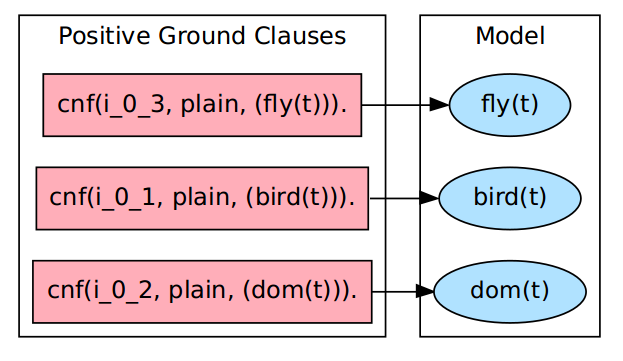
\includegraphics[scale=0.42]{pictures/dot_graph.png}
				\caption{Rendered dot graph of Model\label{fig:dot_graph}}
			\end{figure}
		